\documentclass[10pt,twoside,a4paper,titlepage]{article}
\linespread{1.3}
\usepackage{indentfirst}
\usepackage{amsmath}
\usepackage{graphicx}
\usepackage{fancyhdr}
\usepackage{setspace}
\usepackage[UTF8]{ctex}

\title{EE101 Final Project Report}
\author{Yifu Chen,Jialong Guo , Ziliang Guo, Aofan Jiang}

\begin{document}

\maketitle
\phantom{s}
\thispagestyle{empty}
\clearpage

\tableofcontents
\thispagestyle{empty}
\newpage
\setcounter{page}{1}

\section{Overview}
\subsection{Project File Tree}
	% 
\includegraphics[width=0.7\textwidth]{pics/01.jpg}

\subsection{Develop Environment}


	% Windows 8.1\par
	% XAMPP Version 7.3.2\par
	% MySQL Ver 15.1 Distrib 10.1.38-MariaDB, for Win64 (AMD64)\par
	% Solr 8.0.0\par
	% Browser Google Chrome 74.0.3729.157
	% Editor Sublime Text Version 3.2.1 Build 3027\par
	\newpage
\section{Front-end}
written by Yifu Chen
	%cyf's part
	
	\subsection{Overview}
	
	\subsubsection{Basic Idea}
	
	I was in charge of the front-end part.I mainly used CSS and BOOTSTRAP to beauify our websitek.In my opinion,I hope my websites be plain and straightforward,so I did not decorate our websites deliberately,and this my idea of designing the layout fo our websites.
	
	\subsubsection{Process of development}
	
	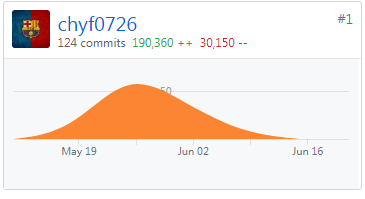
\includegraphics[width=0.7\textwidth]{cyf/contribution.PNG}
	
	We took the advantage of \emph{Github} to promote our cooperation.During the period, I wrote down about 200,000 lines of codes which was mostly written independently,and I was the number 1 contributor in our team.
	
	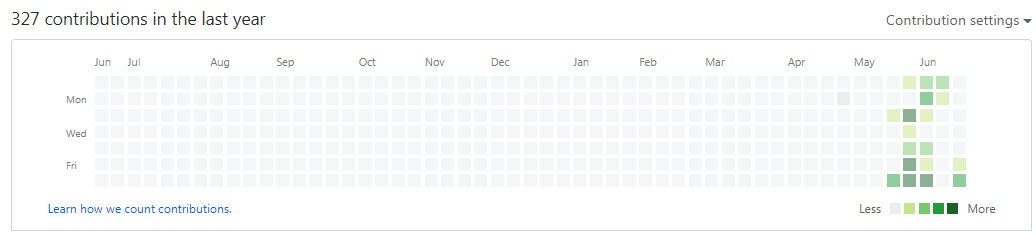
\includegraphics[width=0.7\textwidth]{cyf/frequency.PNG}
	
	I started my job on 26th May and ended on 8th June and I will introduce my job in the following part.
	
	
	\subsection{Index.php}
	
	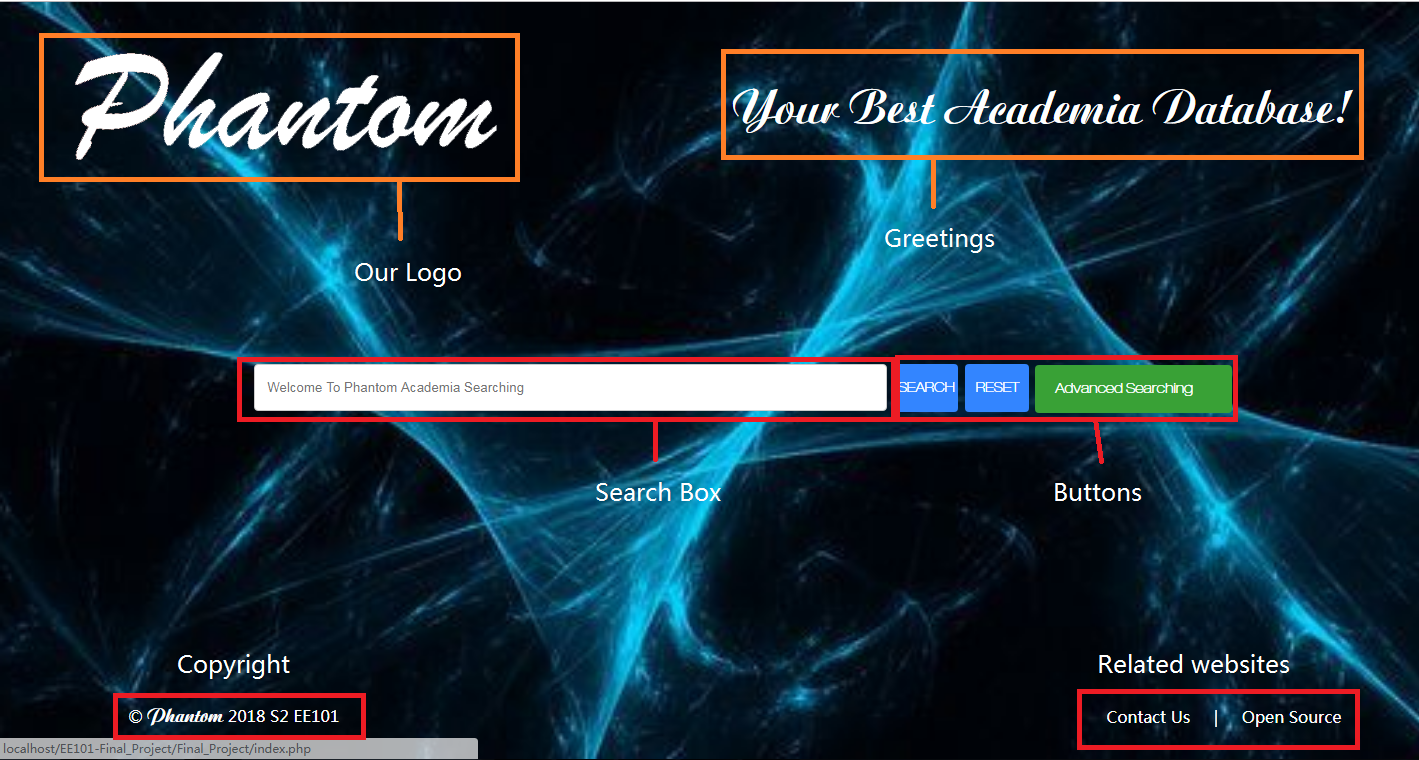
\includegraphics[width=0.7\textwidth]{cyf/index_structure.PNG}
	
	Our index page is shown above.First of all,I would like to introduce the process of my designing our home page.At first,there were three search boxes in the page.The search box "Author","Title" and "conference",and the layout of the index.php was settled.Then,we decided to use multi-searching.Therefore I cut down the number of search boxes into one.Finally,I polished the index.php and the page became what you can see now.
	
	The elements the index page consists of was shown in the graph above,ang I am going to introduce every part respectively.
	
	By the way,the favicon of our websites was \emph{Raffaello}'s \emph{The School of Athens}.
	
	\subsubsection{Logo}
	
	The name of our search engine came from \emph{The Phantom of the opera},one of my favorite films,and I hope that the speed of our searching engine can be as fast as a phantom.It took me so much time to find a appropriate font to display our logo.Finally I found out a font "书体坊兰亭体".However,the words could not be shown in terms of vector graph,which meant that the edge of the words were not smooth,and that is a defect a our logo.
	
	\subsubsection{Greeting Words}
	
	To display the greeting words,I also spent plenty of time to find a approriate fonts.Finally, I found a font named "ChannelSlanted2" to present the greeting words.
	
	\subsubsection{Search box \& buttons}
	
	The search box and the buttons are the key part of the page,and I beautified the buttons,and the result was shown in the following pictures.
	\newline
	\newline
	
\includegraphics[width=0.7\textwidth]{cyf/search1.png}
	\newline
	
\includegraphics[width=0.7\textwidth]{cyf/search2.png}
	\newline
 	
\includegraphics[width=0.7\textwidth]{cyf/search3.png}
 	\newline	
 	
\includegraphics[width=0.7\textwidth]{cyf/search4.png}
 	\newline	
 	
\includegraphics[width=0.7\textwidth]{cyf/search5.png}
 	\newline	
 	
\includegraphics[width=0.7\textwidth]{cyf/search6.png}
 	\newline	
 	
\includegraphics[width=0.7\textwidth]{cyf/search7.png}
 	\newline
	
\includegraphics[width=0.7\textwidth]{cyf/reset1.png}
	\newline
	
\includegraphics[width=0.7\textwidth]{cyf/reset2.png}
	\newline
	
\includegraphics[width=0.7\textwidth]{cyf/reset3.png}
	\newline	
	
\includegraphics[width=0.7\textwidth]{cyf/reset4.png}
	\newline	
	
\includegraphics[width=0.7\textwidth]{cyf/reset5.png}
	\newline	
	
\includegraphics[width=0.7\textwidth]{cyf/reset6.png}
	\newline	
	
\includegraphics[width=0.7\textwidth]{cyf/reset7.png}
	\newline
	
\includegraphics[width=0.7\textwidth]{cyf/Advanced_searching1.png}
	\newline
	
\includegraphics[width=0.7\textwidth]{cyf/Advanced_searching2.png}
	\newline
	
\includegraphics[width=0.7\textwidth]{cyf/Advanced_searching3.png}
	\newline	
	
\includegraphics[width=0.7\textwidth]{cyf/Advanced_searching4.png}
	\newline	
	
\includegraphics[width=0.7\textwidth]{cyf/Advanced_searching5.png}
	\newline	
	
\includegraphics[width=0.7\textwidth]{cyf/Advanced_searching6.png}
	\newline	
	
\includegraphics[width=0.7\textwidth]{cyf/Advanced_searching7.png}
	\newline
	
\includegraphics[width=0.7\textwidth]{cyf/Advanced_searching8.png}
	\newline
	
\includegraphics[width=0.7\textwidth]{cyf/Advanced_searching9.png}
	\newline
	
\includegraphics[width=0.7\textwidth]{cyf/Advanced_searching10.png}
	\newline	
	
\includegraphics[width=0.7\textwidth]{cyf/Advanced_searching11.png}
	\newline	
	
\includegraphics[width=0.7\textwidth]{cyf/Advanced_searching12.png}
	\newline	
	
\includegraphics[width=0.7\textwidth]{cyf/Advanced_searching13.png}
	\newline	
	
\includegraphics[width=0.7\textwidth]{cyf/Advanced_searching14.png}
	\newline	
	
\includegraphics[width=0.7\textwidth]{cyf/Advanced_searching15.png}
	\newline	
	
\includegraphics[width=0.7\textwidth]{cyf/Advanced_searching16.png}
	\newline	
	
\includegraphics[width=0.7\textwidth]{cyf/Advanced_searching17.png}
	\newline	
	
\includegraphics[width=0.7\textwidth]{cyf/Advanced_searching18.png}
	\newline	
	
\includegraphics[width=0.7\textwidth]{cyf/Advanced_searching19.png}
	\newline	
	
\includegraphics[width=0.7\textwidth]{cyf/Advanced_searching20.png}
	\newline	
	
\includegraphics[width=0.7\textwidth]{cyf/Advanced_searching21.png}
	\newline	
	
\includegraphics[width=0.7\textwidth]{cyf/Advanced_searching22.png}
	\newline	
	
\includegraphics[width=0.7\textwidth]{cyf/Advanced_searching23.png}
	\newline	
	
\includegraphics[width=0.7\textwidth]{cyf/Advanced_searching24.png}
	\newline	
	
\includegraphics[width=0.7\textwidth]{cyf/Advanced_searching25.png}
	\newline	
	
\includegraphics[width=0.7\textwidth]{cyf/Advanced_searching26.png}
	\newline	
	
\includegraphics[width=0.7\textwidth]{cyf/Advanced_searching27.png}
	\newline	
	
\includegraphics[width=0.7\textwidth]{cyf/Advanced_searching28.png}
	\newline	
	
\includegraphics[width=0.7\textwidth]{cyf/Advanced_searching29.png}
	\newline	
	
\includegraphics[width=0.7\textwidth]{cyf/Advanced_searching30.png}
	\newline	
	
\includegraphics[width=0.7\textwidth]{cyf/Advanced_searching31.png}
	
	\subsubsection{Copyright \& Related Websites}
	
	These two parts were mainly written by Ziliang Guo and Aofan Jiang and Hyperlinks were set on the texts "Contact Us" and "Open source".
	
	\subsection{Search.php}
	
	I am going to introduce every part of search.php respectively.
	\newline
	
	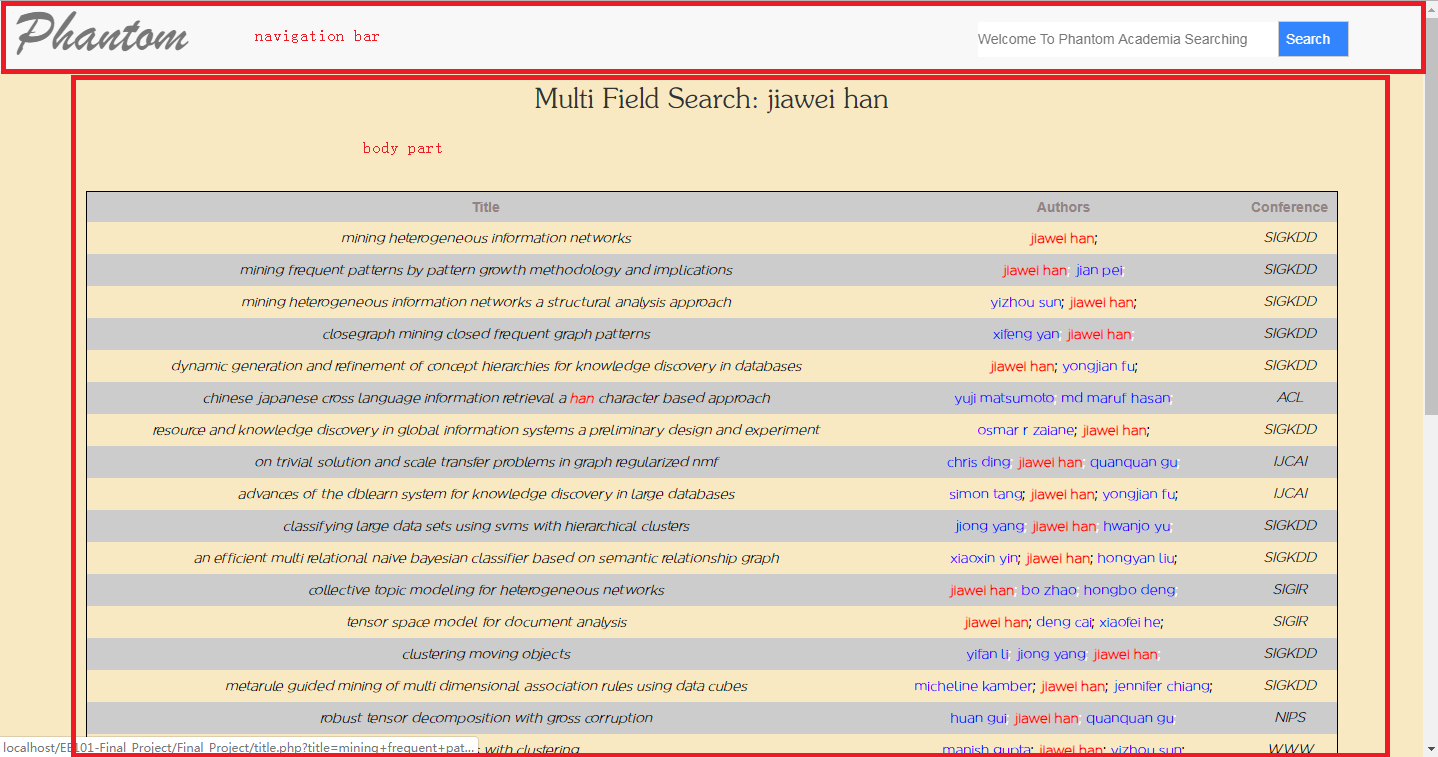
\includegraphics[width=1.0\textwidth]{cyf/SEARCH_struct1.png}
	\newline
	\includegraphics[width=1.0\textwidth]{cyf/SEARCH_2_struct2.png}
	
	
	\subsubsection{Navigation Bar}
	
	I used css and bootstrap to construct the navigation bar.I thought there was no need to build a  that complicated navigation bar,so I just put our logo in the top left corner of the screen and set it with a hyperlink to the homepage,and in the top right corner if the screen was a search box to conduct multi-search.
	
	\subsubsection{Body Part \& Text}
	
	I selected the font "Regencie" to beaufy the table and "书体坊赵九江钢笔楷书" to beatufy the texts.
	
	\subsubsection{Paper Turning \& "Jump to" Button }
	
	Our idea to design the pattern of the Paper Turning is to imitate \emph{Google}'s pattern.
	
	\includegraphics[width=0.5\textwidth]{cyf/Google.jpg}
	
	Therefore,I photoshopped some pictures and realized this idea.
	
	I beautfied the "Jump to" box,and the button "Go!" was modified by Aofan Jiang.
	
	
	\subsection{Conference.php}

 \hspace*{\fill} 
\begin{flushleft}
	\includegraphics[width=1.0\textwidth]{cyf/Conference.PNG}
	\newline
	
	\includegraphics[width=1.0\textwidth]{cyf/Conference2.PNG}
\end{flushleft}

	The beautification of Conference.php was similiar to the search.php.Therefore I will not go into details here.
	
	\subsection{Author.php}
	
	 \hspace*{\fill} 
	\begin{flushleft}
		\includegraphics[width=1.0\textwidth]{cyf/author1.PNG}
		\newline
		
		\includegraphics[width=1.0\textwidth]{cyf/author2.PNG}
	\end{flushleft}

	The beautification of the page author was similiar to the search.php.Therefore I will not go into details here as well.
	
	\subsection{Title.php}
	
	
	
	
	
	
	
	
	
	
	
	
		
	
	
	
	
	
	
		
	
	 
	
	
	



% ----------  BEGIN  ------------
% GJL
% ------>	

\newpage

	\section{Graphs}
		\textbf{\emph{[Start] --- By Jialong Guo 518030910272 ---}}\newline\par

	\subsection{Overview}
		\includegraphics[width=0.9\textwidth]{gjl/overview.jpg}\newline\par
		When it comes to our graph part, it can be chiefly divided into three parts: \newline \par
		The first of which is to get all the data we need in order to draw a graph.\newline\par
		The second part of which is to format all the data into the form that the corresponding graph is needed.\newline\par
		The last part of which is just to use specific javascript library to create graphs and make them beautiful. \newline\par

	\subsection{Design}
		\par In author page’s left part, I add a collumn graph, which displays the number of publication the author has yearly and
shows the trend of his/her academic activity to give users a clear impression about the author’s research fruit and the frequency of his/her delivery.
		\par In author page’s left part, I also add a pie graph, which showcases how many papers the author publishs in a conference which brings a clear view on the author is mostly connected with what conference.
		\par In paper page's upper part, there’s a line-collumn graph showing its yearly citations, from which we can gain a insight into the popularity of its research field.
		\par In paper page's lower part, I use a force directed graph to display the relations between similar papers. It gives a convience way to find related papers and messages.
		\par In conference page, a line graph of its yearly amount of papers may reveal its academic influence.

	\subsection{Searching Data}
		\par In this subsection I mainly discuss the first part of graph drawing, get data from database. Since diverse graphs need diverse data, here I just demonstrate a specific example of getting data, which can mostly stand for my means of searching data.
		\subsubsection{From Mysql to Solr}
			\par Taking time cost into consideration, we may need to import data into solr from mysql in advance, for searching from solr will spend more time than from mysql. Thereby, it is required that we write the referenceID of reference papers into solr's schema, which allows us to search the reference papers of a paper just from solr when needed.
			\par The final data we put in solr is formed in this way:\newline\par
			\includegraphics[width=0.9\textwidth]{gjl/formdata.jpg}\newline\par
		You can refer to the codes attached for detailed information.
		\subsubsection{Searching in Solr}
			\par The first step is getting value form user's input, then create the url link to search in solr. After this step, we can get a .json file with the result.

	\subsection{Formatting Data}
		\par In this section, we mainly discuss how to change the search result into suitable formation of drawing a graph. 

	\subsection{Drawing Graph}
		\par In the section, the process of drawing with echarts is mainly discussed.

	\subsection{Fruits' Display}
		\includegraphics[width=0.4\textwidth]{gjl/11.jpg}\newline\par
		\includegraphics[width=0.4\textwidth]{gjl/12.jpg}\newline\par
		\includegraphics[width=0.4\textwidth]{gjl/21.jpg}\newline\par
		\includegraphics[width=0.4\textwidth]{gjl/22.jpg}\newline\par
		\includegraphics[width=0.4\textwidth]{gjl/3.jpg}\newline\par

		\textbf{\emph{[End] --- By Ziliang Guo 518030910273 ---}}

		
% <------
% GJL
% ----------   END   ------------


\newpage


% ----------  BEGIN  ------------
% GZL
% ------>	

	\section{Overview}
		\textbf{\emph{[Start] --- By Ziliang Guo 518030910273 ---}}\newline\par
		(1) I took the initiative that we take full advantage of Github to accelerate our project. I also create a document to take notes of the porblems we met and the solutions.\newline\par
		(2) Actually, I wrote the manual and uploaded my Lab 01 - 03 codes to unify the databases.\newline\par
		(3)	I mainly focus on the back-end development.\newline\par
		(4) Of all my codes, I wanna highlight that approximately 85\% are mainly created  independently. For the remaining codes, modification is applied, with reference to some online blogs.\newline\par
		(5) Meanwhile, during my coding, I always remember to leave interfaces for my collaborators.\newline\par
		(6)	As is vividly depicted in the timeline graph, I realized and improved different sections separately, in other words, term by term. Of course, my constant improvements are shown.\newline\par
		\includegraphics[width=0.9\textwidth]{gzl/01.png}


	\section{Keyword Highlighting}
		I adopted the “hl” settings of Solr. It is somehow very simple. Just echo the corresponding urls will do.\par
		However, please notice that, for multivalued fields such as Authors\_Name, only the highlighted part is returned. So I made judgements in such special cases.\newline\par
		Codes:\newline\par
		\includegraphics[width=0.9\textwidth]{gzl/02.jpg}


		% 4.	Page Turning
		% Now, here comes the page turning part. It appears in several pages, namely, search, author, conference, advanced search. Actually, this part undergoes about three versions, and you guys can see the V2.0 and the advanced version.

		% As for the features of the versions:
		% Hyperlink means that I use hyperlinks to jump to a new page.
		% Anchor refers to the fact that after turning pages, the page will be automatically guided to the titles of the result tables for better user experience.
		% Jump to stands for the jump-to function, which enables users to jump to a valid page of results.
		% Actually, the 2.0 and higher version, I tried to imitate the page-turning function of Google. But for the methods, improved hyperlinks for the former, while Jquery and Ajax for the latter.


		% As you can see, the current page is highlighted in red and the red u cannot be clicked.
		% Previous page and next page buttons appear if and only if such a page is applicable.

		% The simple search V1.0 is just that of my Lab03. It’s simple and sometimes naïve.
		% For the V2.0, multi-field search is applied. All the results, containing the target keywords in Fields Title, Authors_Name, and Conference, will be displayed. These fields are of the same importance. By the way, I designed some widgets.
		% Now let’s have a look at the webpages.
		% (Open the browser)

		% I also implemented some tiny webpage features.
		% For all the pages, after refreshing, the page will jump to the location where the user was previously browsing.
		% Still, for all the pages, if a hyperlink is clicked, the new page will be opened in a new window.
		% In addition, I improved the loading speed of the author page.

		% Paper recommendation in academic formats, which can be hidden and shown, is available on the title page.
		% The order and weight account for three parameters. Cited times are given top priority, followed by authors and title. The authors of a certain paper are given a descending weight and the weight of the title is similar to that of the first author.
		% (Open the browser)


		% The advanced search is key to a good search engine.
		% This page is made separately using Jquery and Ajax. A slowly descending The keywords are given a slowly descending weight.


		% We value users’ precious feedbacks. So we add a feedback page.
		% The unfilled blanks will be alerted and the pending status will be clearly illustrated. What’s more, the log will be saved locally. I take advantage of NodeJS and emailjs to implement the function.
		% Considering the network and the fact that this function is still a beta version, probably the outcome is not that satisfactory. But, does anybody wanna have a try?

	\textbf{\emph{[End] --- By Ziliang Guo 518030910273 ---}}
% <------
% GZL
% ----------   END   ------------

\newpage

% ----------  BEGIN  ------------
% JAF
% ------>	

\section{Hyperlinks}
\textbf{\emph{--- By Aofan Jiang 518030910275 ---}}\newline\par
As required in the final project, I add the hyperlink of each title, author and conference. So the users can click to get more information about the result they want to search for.
\subsection{Hyperlink of each title}
Different from the table about the information of key words, the title page is simply a series of main information about the corresponding paper. It includes the paper ID, the publish year, the authors, conference name, and reference papers. This can make the whole page clearer,just as the following picture.\newline\par
\includegraphics[width=0.9\textwidth]{jaf/titleexample.PNG}\newline\par
 It might be ignored that the table of reference paper title of each paper is given in the original data. Although it is not required in the lab two, I still add it as a field in Solr to make sure that more detailed information can be gotten by the users. This explains the existence of references in the paper page.\newline\par
What’s more, to make a user-friendly website, you can see in the following picture that at the top of website, the link information about the title. It’s also clear and easy to find the information. It’s linked by the symbol of addition.\par
\includegraphics[width=0.9\textwidth]{jaf/link.PNG}\newline\par
 On the comparison, you can see even in Baidu NetDisk that the link is not so comfortable as ours. They are all connected with \%2 while our website link are connected with + . Since all the information is imported in solr, the searching speed is quite fast with no delay.\par
\includegraphics[width=0.9\textwidth]{jaf/linked.PNG}\newline\par
\subsection{Hyperlink of each conference}
This page is also mainly an information table like the main searching page. It includes each paper’s title, authors published on the given conference name. However, at the last column of table, the original conference name is replaced by the publish year of each paper published in this conference.\par
\includegraphics[width=0.9\textwidth]{jaf/conference.PNG}\newline\par
\subsection{others}
Even at different pages among paper, author, conferences. Almost all the items are hyperlinked. So it means you can jump to different pages in any given page. Here comes an example of authors' information\par
\includegraphics[width=0.9\textwidth]{jaf/author.PNG}\par

\section{Code optimization}
\subsection{Solr}
By testing, I find that the searching speed by solr is faster than mysql. So all the places that can be used in solr are changed from mysql.\par
\subsection{Mysql}
When using mysql, there are still some methods to improve the speed of program.\par If the searching result is only one piece. For instance, the publish year, the affiliation and the conference and so on. We can limit the searching result numbers by add the code “LIMIT 1 ”. As a result, when mysql get one information about the result, it will stop the searching process, which is a great improvement in the speed of a program.\par
\includegraphics[width=0.9\textwidth]{jaf/limit.PNG}\newline\par
 Instead of using inner join, try to use more simple searching and output the result together is faster.\par
\includegraphics[width=0.9\textwidth]{jaf/affold.PNG}\newline\par
\includegraphics[width=0.9\textwidth]{jaf/affnew.PNG}\newline\par
As for the code in php, we can choose to use mysqli\_fetch\_row rather than mysqli\_fetch\_array since the information class is of each column is known to us.\par

\section{Contact and Open source}
At the home page, you can find the word “contact us ”. After clicking it, you will jump to a new page with a sophisticated chart. You can input your information and your information, we will get your feedback after you clicking the submit button.\newline\par
\includegraphics[width=0.9\textwidth]{jaf/contact.PNG}\newline\par
Also, you can find the word ”open source ”. After clicking it, you will jump to our project on Github website. At here, you can check all the detailed codes and corresponding documents.\newline\par
\includegraphics[width=0.9\textwidth]{jaf/git.PNG}\newline\par
\newpage

% <------
% JAF
% ----------   END   ------------




\end{document}